\documentclass[11pt,parskip=half,a4paper]{scrartcl}
%\usepackage{ngerman}
\usepackage[latin9]{inputenc}
\usepackage[T1]{fontenc}
\usepackage{multicol}
\usepackage{graphicx}
\usepackage{pslatex}
\usepackage{helvet}
\usepackage{listings}
\lstset{numbers=left, numberstyle=\tiny, numbersep=4pt, breaklines=true, frame=single, showstringspaces=false, basicstyle=\scriptsize}
% -*- latex -*-
% Definition of the Lua language for the listings package
% Time-stamp: <2008-11-30 15:27:16 rsmith>
% Written by Roland Smith <rsmith@xs4all.nl> and hereby placed in the public
% domain. 

\lstdefinelanguage{lua}
  {morekeywords={and,break,do,else,elseif,end,false,for,function,if,in,local,
     nil,not,or,repeat,return,then,true,until,while},
   morekeywords={[2]arg,assert,collectgarbage,dofile,error,_G,getfenv,
     getmetatable,ipairs,load,loadfile,loadstring,next,pairs,pcall,print,
     rawequal,rawget,rawset,select,setfenv,setmetatable,tonumber,tostring,
     type,unpack,_VERSION,xpcall},
   morekeywords={[2]coroutine.create,coroutine.resume,coroutine.running,
     coroutine.status,coroutine.wrap,coroutine.yield},
   morekeywords={[2]module,require,package.cpath,package.load,package.loaded,
     package.loaders,package.loadlib,package.path,package.preload,
     package.seeall},
   morekeywords={[2]string.byte,string.char,string.dump,string.find,
     string.format,string.gmatch,string.gsub,string.len,string.lower,
     string.match,string.rep,string.reverse,string.sub,string.upper},
   morekeywords={[2]table.concat,table.insert,table.maxn,table.remove,
   table.sort},
   morekeywords={[2]math.abs,math.acos,math.asin,math.atan,math.atan2,
     math.ceil,math.cos,math.cosh,math.deg,math.exp,math.floor,math.fmod,
     math.frexp,math.huge,math.ldexp,math.log,math.log10,math.max,math.min,
     math.modf,math.pi,math.pow,math.rad,math.random,math.randomseed,math.sin,
     math.sinh,math.sqrt,math.tan,math.tanh},
   morekeywords={[2]io.close,io.flush,io.input,io.lines,io.open,io.output,
     io.popen,io.read,io.tmpfile,io.type,io.write,file:close,file:flush,
     file:lines,file:read,file:seek,file:setvbuf,file:write},
   morekeywords={[2]os.clock,os.date,os.difftime,os.execute,os.exit,os.getenv,
     os.remove,os.rename,os.setlocale,os.time,os.tmpname},
   sensitive=true,
   morecomment=[l]{--},
   morecomment=[s]{--[[}{]]},
   morestring=[b]",
   morestring=[d]'
  }

\lstset{language=lua}
\usepackage[pdftitle={HeliTrim Manual},pdfstartview={FitH},colorlinks=true]{hyperref}
\pdfcompresslevel=9
\pdfimageresolution=72

\usepackage{color}
\definecolor{hellgrau}{gray}{0.85}
\definecolor{dunkelgrau}{gray}{0.55}

\newcommand{\hinweis}[2]{%
\phantomsection\addcontentsline{toc}{section}{#1}
\begin{center}
\fcolorbox{dunkelgrau}{hellgrau}{\parbox{14cm}{\textbf{#1}#2}}
\end{center}
}

\newcounter{aufg}
\newcommand{\xsb}{XSquawkBox}
\newcommand{\punkte}[1]{\marginpar{\fcolorbox{dunkelgrau}{hellgrau}{\parbox{4.5ex}{\sffamily\tiny#1}}}}

\renewcommand{\labelenumi}{\alph{enumi})}

\newcommand{\aufgabe}{\stepcounter{aufg}\vspace{0.75cm}\pagebreak[3]{\phantomsection\addcontentsline{toc}{section}{Aufgabe~\arabic{aufg}}\Large\sffamily Aufgabe~\arabic{aufg}}}
\renewcommand{\labelenumi}{\alph{enumi})}

\usepackage{fancyhdr}
\usepackage{lastpage}
\pagestyle{fancy}

\setlength{\headheight}{2cm}
%\chead{\includegraphics[width=2.0cm]{FlyWithLua_logo.jpg}\\[2ex]}
\cfoot{\footnotesize Page \thepage\ of \pageref{LastPage}}
\renewcommand{\headrulewidth}{0.4pt}
\renewcommand{\footrulewidth}{0.4pt}

\begin{document}

\title{Xbtn2cmd Reference Manual}
\author{William Good}
\date{\today}

\maketitle
\vspace{2cm}

\begin{center}
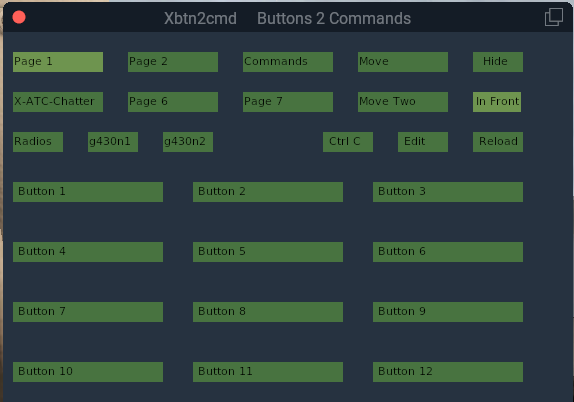
\includegraphics[width=15cm]{Xbtn2cmd_Page1.png}
\end{center}

\thispagestyle{empty}
\newpage
\verb||
\tableofcontents

\newpage
\section{Introduction}

When I started using VR I was only using the touch controllers and I found out that I need some way to replicate the missing buttons from a joystick or yoke. This is the solution I have came up with and has went through a few versions refining it to match my needs. \newline

Since the updated SDK came out supporting VR it allowed creating new "modern" window styled like an X-Plane 11 window. This allowed a new GUI window with 12 blank buttons per page that you can label and add commands to the buttons. It allows you to have 8 pages of buttons that the page button can be labeled and is highlighted when selected. 

\section{How to Install}
To Install copy the Xbtn2cmd folder from the archive into the Resources/plugins folder. \newline

When X-Plane starts go to the Plugins > Xbtn2cmd > Toggle Window and then the window will be displayed. \newline

You can also map a command (bgood/xbtn2cmd/toggle\_window) to Toggle Xbtn2cmd to be visable. \newline

There is a xbtn2cmd.ini file that for each button has "pagex\_button1\_label" and "pagex\_button1\_command" located in the Xbtn2cmd folder where x is page1 thru page8. \newline

"pagex\_button1\_label" allows you to label the button and "pagex\_button1\_command" allows you to give the button a command to do when the button is clicked. \newline

You can also make a copy of xbtn2cmd.ini and put it in the aircraft folder the same place where the *.acf file is. This will allow a custom xbtn2cmd.ini for each aircraft you fly. If you have more that one *.acf in the aircraft folder you can also use the aircraft name and the suffix \_xbtn2cmd.ini so for the default Cessna is would be Cessna\_172SP\_xbtn2cmd.ini. \newline

If you are editing the xbtn2cmd.ini file on Windows please use notepad++ that can be found here https://notepad-plus-plus.org/.

\section{Pages}

\begin{center}
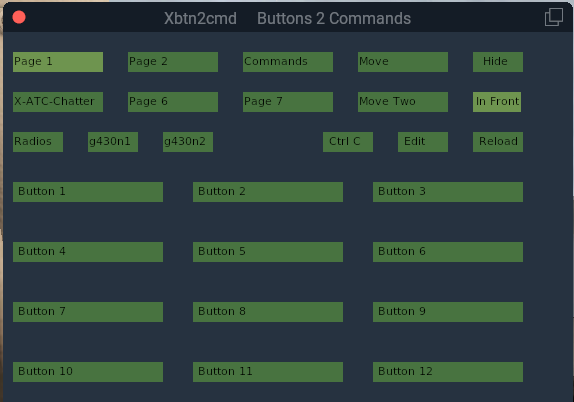
\includegraphics[width=15cm]{Xbtn2cmd_Page1.png}
\end{center}

Whenever you have selected any of the eight big buttons at the top of the window a different set of twelve buttons are displayed in the lower part of the window. The page buttons labels and the button labels can all be changed to match what you want. What commands the buttons do can also be configured including once and continue. \newline

The hide button just hides the window if you no longer need it. The In Front indicator let you know if the window will accept mouse clicks and must be highlighted to accept them but clicking anywhere on the window will highlight it. The reload button will reload the *.ini file after changes have been made to it and you will see the changes displayed on the buttons. The other buttons are are described later in the manual with there own sections. 

\newpage
\section{Radios Page}

\begin{center}
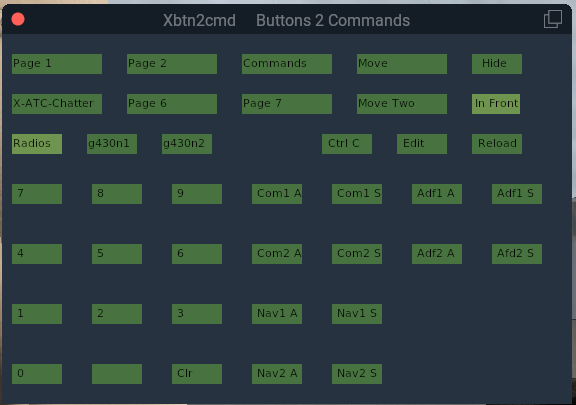
\includegraphics[width=15cm]{Xbtn2cmd_Radios_Page.png}
\end{center}

The radios page lets you to quickly set com, nav and adf frequencies. You do this by using the provided keypad to enter the proper frequency. For com and nav that is five digits that is displayed on the bottom row just after the zero key. For adf it is four digits and if you want to enter three then lead with a zero. Once you have entered the proper frequency click on the type you want to set. There is a Clr button to clear out any errors you might have made to start over. When you have made your choice the entry display window is cleared. \newline

Because of the nature of this page none of the button labels can be changed.

\newpage
\section{g430n1 X-Plane 530 Page}

\begin{center}
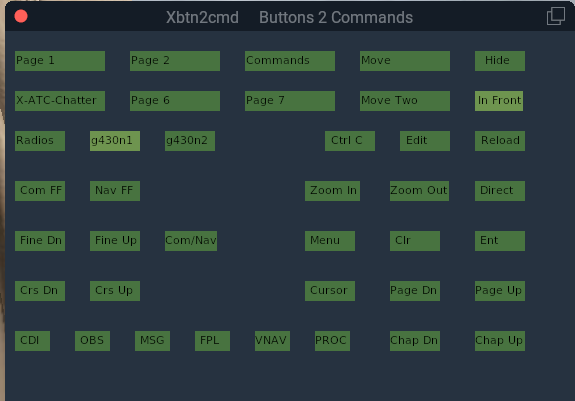
\includegraphics[width=15cm]{Xbtn2cmd_g430n1_530_Page.png}
\end{center}

If you are having trouble using the touch controllers to click on the buttons or turn the knobs for the X-Plane 530 in the VR cockpit this might make it easier for you. \newline

Because of the nature of this page none of the button labels can be changed.

\newpage
\section{g430n2 X-Plane 430 Page}

\begin{center}
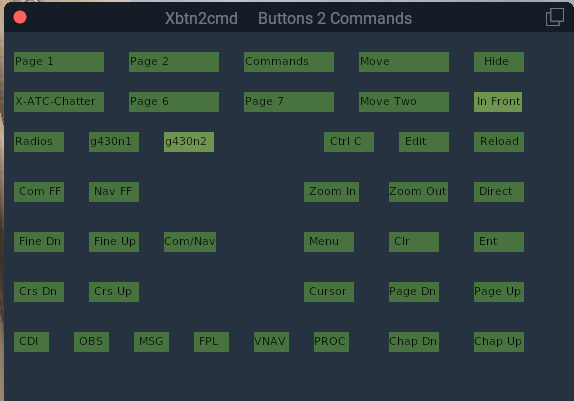
\includegraphics[width=15cm]{Xbtn2cmd_g430n2_430_Page.png}
\end{center} 

If you are having trouble using the touch controllers to click on the buttons or turn the knobs for the X-Plane 430 in the VR cockpit this might make it easier for you. \newline

Because of the nature of this page none of the button labels can be changed.

\newpage
\section{Edit Page}

\begin{center}
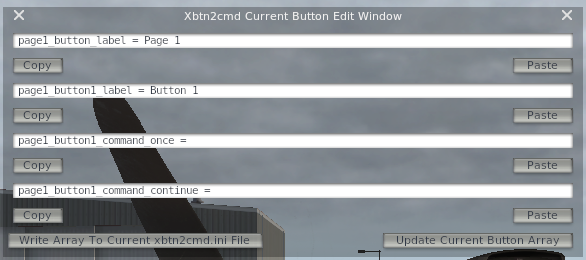
\includegraphics[width=15cm]{Xbtn2cmd_Edit_Page.png}
\end{center}

The edit page allows you to change the label and commands and can be opened by pressing the Edit button. It has copy and paste buttons to allow you to paste a command or label from the clipboard into the field of your choice. After you have made your changes in the edit fields then click on the "Update Current Button Array". Next click on the "Write Array to Current xbtn2cmd.ini File" button to save your changes and then click on the Reload button to see your changes reflected on the window. 

\section{Ctrl C button}

To edit in VR I have added a delayed Control C to allow copying of items in another window. To use this press on the Ctrl C button and you will hear Control C in 10 seconds. At that point highlight want you want to be put in the clipboard before 10 seconds is up. After 10 seconds you will hear Control C now at which point it will execute the command. I have found this to be the most effective method to to a copy while being in VR.

\newpage
\section{Helpful Programs}

One program that I use constantly with Xbtn2cmd is DataRefTool and thanks to Lee Baker for creating this. Now that it has support fo VR I do not have to take off my headset and can fully configure Xbtn2cmd while in VR.

A second program is FlyWithLua created by Carsten Lynker that can be used to expand what is possible with Xbtn2cmd just like I used it with my Xsaitekpanels. I will be providing a scripts to allow using one button to do more than one command. 

\end{document}
